\documentclass[11pt]{article}
\usepackage[margin=2.5cm]{geometry}
\usepackage[utf8]{inputenc}
\usepackage[T1]{fontenc}
\usepackage{graphicx}
\graphicspath{{figures/}{../code/figures/}}
\usepackage{float}
\usepackage{amsmath}
\usepackage{amssymb}
\usepackage{booktabs}
\usepackage{xcolor}
\usepackage{listings}
\usepackage{hyperref}

\lstset{basicstyle=\ttfamily\small, columns=fullflexible, keepspaces=true,
        frame=single, breaklines=true, showstringspaces=false}

% Figures referenced in this document (upload to figures/ in the Overleaf project):
%   a2_weekly_hist.png  a2_weekly_returns_vol.png  a2_weekly_volume.png  a2_weekly_corr.png
%   a2_weekly_lag_box.png  a2_weekly_up_share.png  a2_auto_boxplots.png  a2_auto_corr.png
%   a2_bootstrap_prob.png
%
% Handwritten solutions: \handwritten{a.jpg,b.png,...} shows the first of the listed
% files that exists, in figures/ or in the project root. Until one exists, a placeholder
% box is shown.
\makeatletter
\newcommand{\handwritten}[1]{%
  \def\hw@found{}%
  \@for\hw@file:=#1\do{%
    \ifx\hw@found\@empty
      \IfFileExists{figures/\hw@file}{\edef\hw@found{\hw@file}}{%
        \IfFileExists{\hw@file}{\edef\hw@found{\hw@file}}{}}%
    \fi}%
  \ifx\hw@found\@empty
    \begin{center}\fbox{\parbox{0.9\linewidth}{\centering\vspace{3em}
      Handwritten solution: upload \texttt{\detokenize{#1}} to \texttt{figures/}\vspace{3em}}}\end{center}%
  \else
    \begin{center}\includegraphics[width=\linewidth,height=0.85\textheight,keepaspectratio]{\hw@found}\end{center}%
  \fi}
\makeatother
\newcommand{\todo}[1]{\textcolor{red}{\textbf{TODO:} #1}}

\title{MATH 4432 -- Assignment 2}
\author{Erik Jin}
\date{October 2026}

\begin{document}
\maketitle

\noindent Chapter 4: exercises 1, 2, 3, 13, 14. Chapter 5: exercises 1, 2, 5, 6.
The code and full output are in the notebook \texttt{MATH\_4432\_Assignment\_2.ipynb}.

% ============================================================================
\section*{Chapter 4}

\subsection*{Exercises 1 and 2}
\handwritten{ch4_ex1.jpg}

\subsection*{Exercise 3}
\handwritten{ch4_ex3.jpg}

% ----------------------------------------------------------------------------
\subsection*{Exercise 13 -- \texttt{Weekly}}

\subsubsection*{(a) Numerical and graphical summaries.}

\begin{table}[H]
  \centering
  \begin{tabular}{lr}
    \toprule
    & \texttt{Today} \\
    \midrule
    Mean & 0.150 \\
    Standard deviation & 2.357 \\
    Skewness & $-0.481$ \\
    Excess kurtosis & 5.685 \\
    Share of Up weeks & 0.556 \\
    \bottomrule
  \end{tabular}
  \caption{Summary of the weekly return \texttt{Today} (1\,089 weeks, 1990--2010).}
\end{table}

\begin{figure}[H]
  \centering
  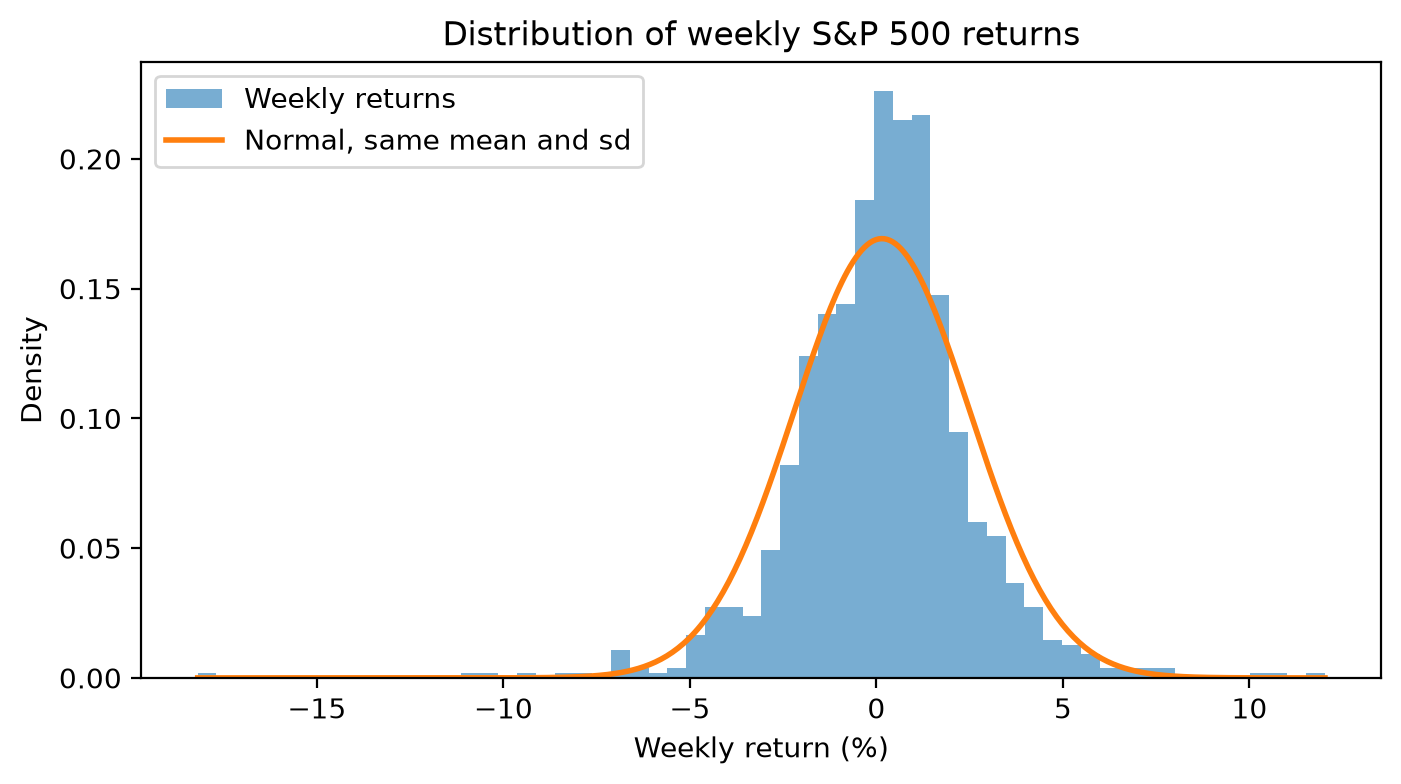
\includegraphics[width=0.75\linewidth]{a2_weekly_hist.png}
  \caption{Distribution of weekly returns with a normal density of the same mean and standard deviation.}
\end{figure}

\begin{figure}[H]
  \centering
  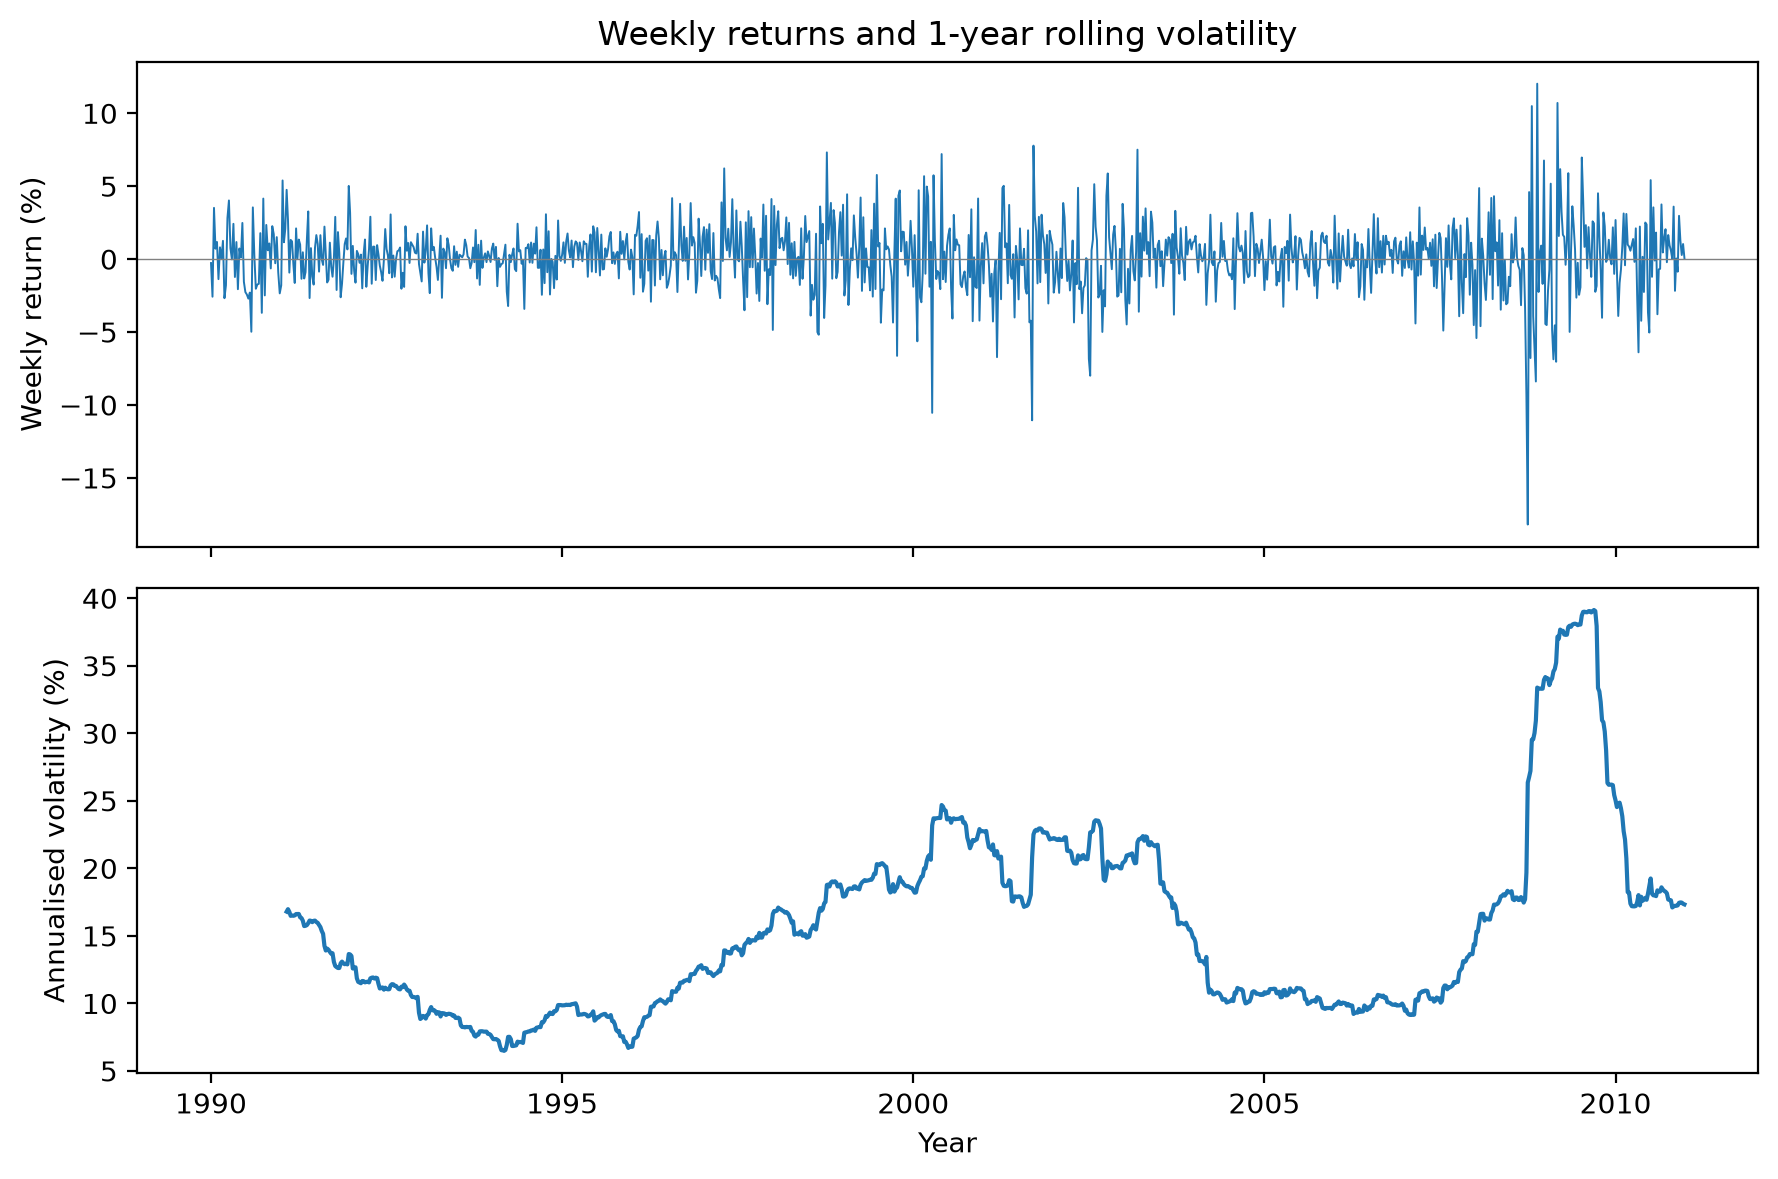
\includegraphics[width=0.85\linewidth]{a2_weekly_returns_vol.png}
  \caption{Weekly returns (top) and 1-year rolling volatility, annualised (bottom).}
\end{figure}

\begin{figure}[H]
  \centering
  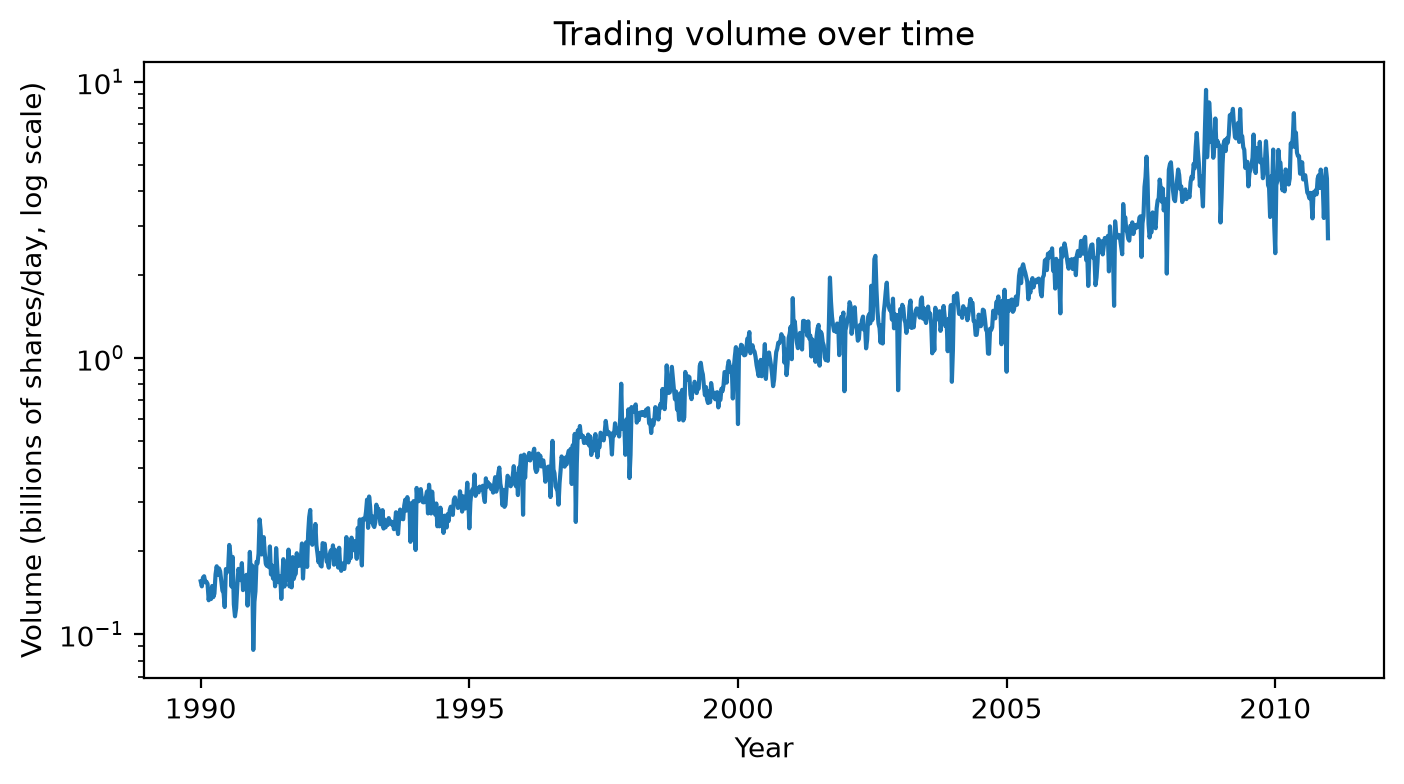
\includegraphics[width=0.75\linewidth]{a2_weekly_volume.png}
  \caption{Trading volume over time (log scale).}
\end{figure}

\begin{figure}[H]
  \centering
  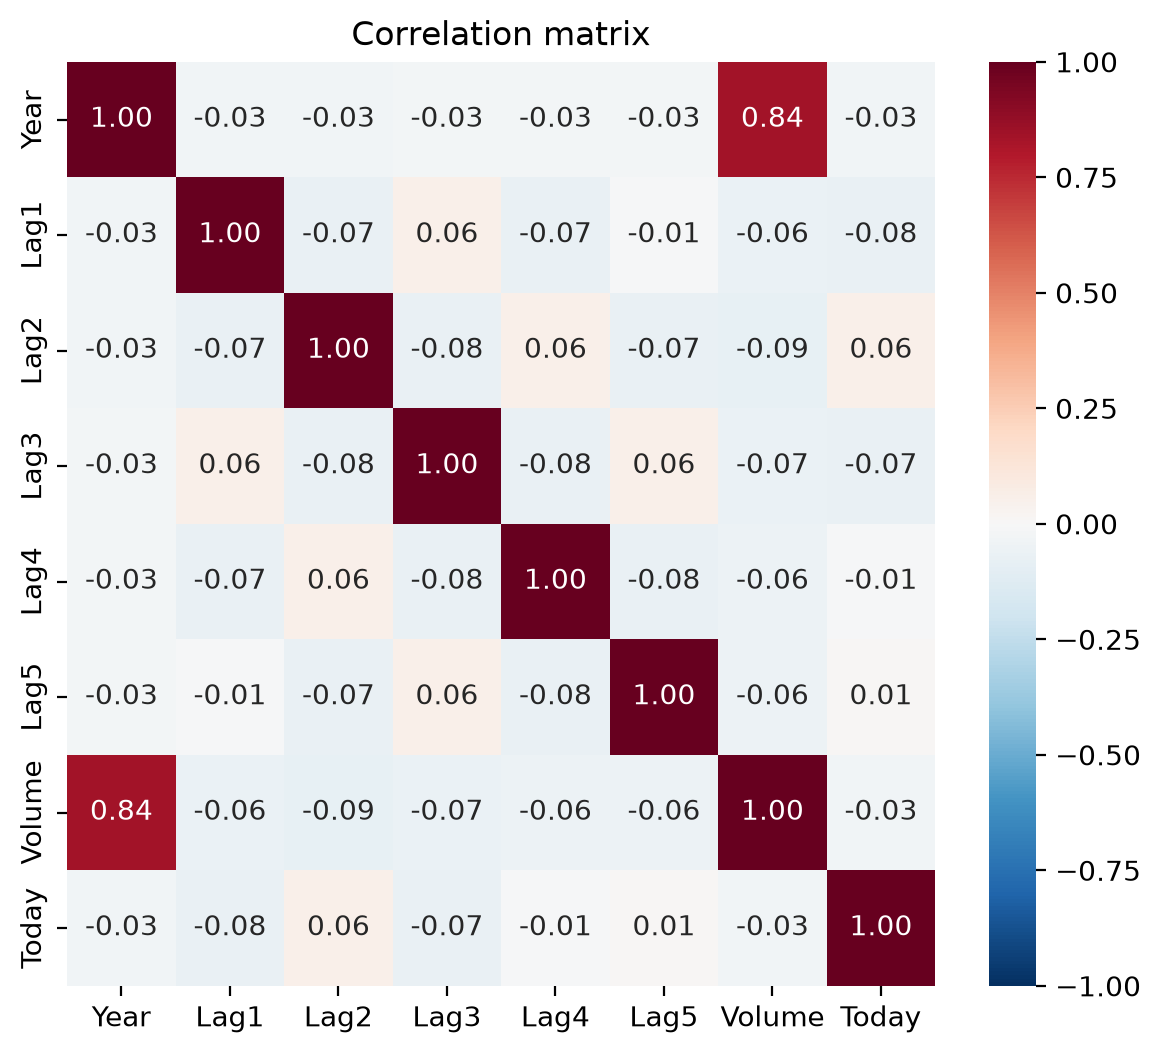
\includegraphics[width=0.6\linewidth]{a2_weekly_corr.png}
  \caption{Correlation matrix of the quantitative variables.}
\end{figure}

\begin{figure}[H]
  \centering
  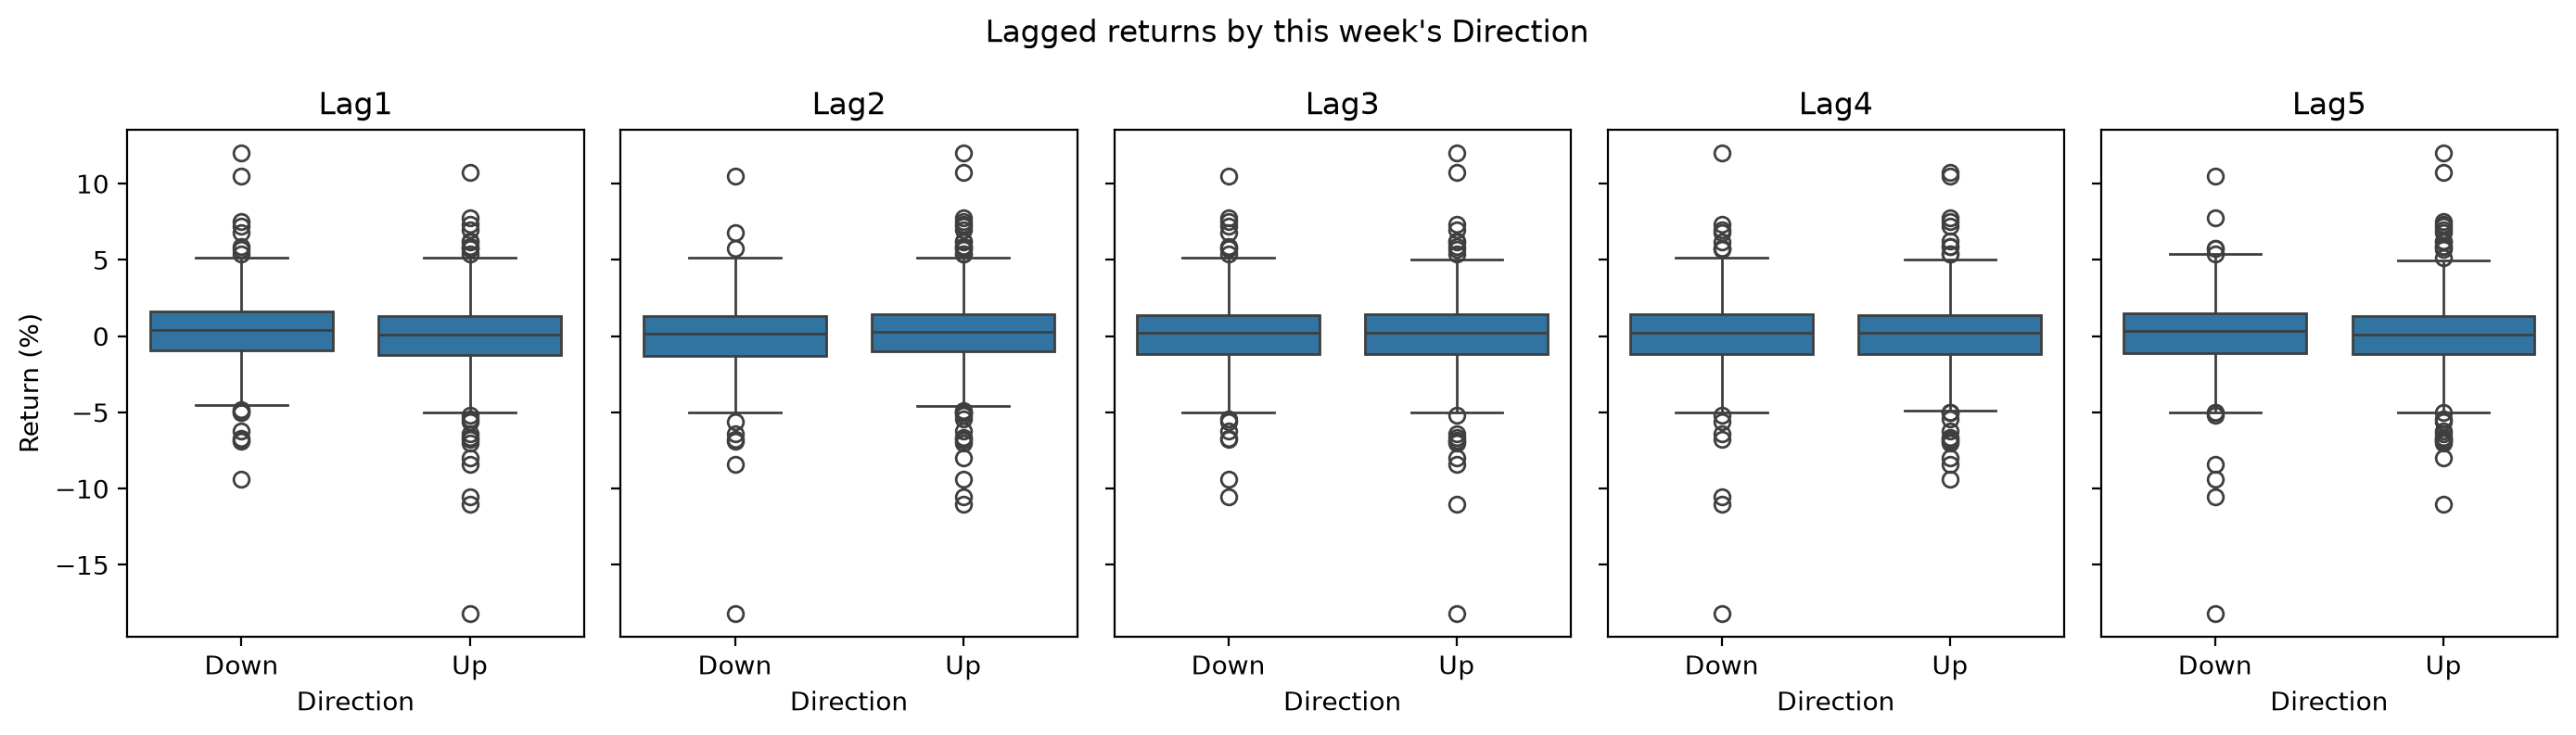
\includegraphics[width=\linewidth]{a2_weekly_lag_box.png}
  \caption{Lagged returns by this week's \texttt{Direction}.}
\end{figure}

\begin{figure}[H]
  \centering
  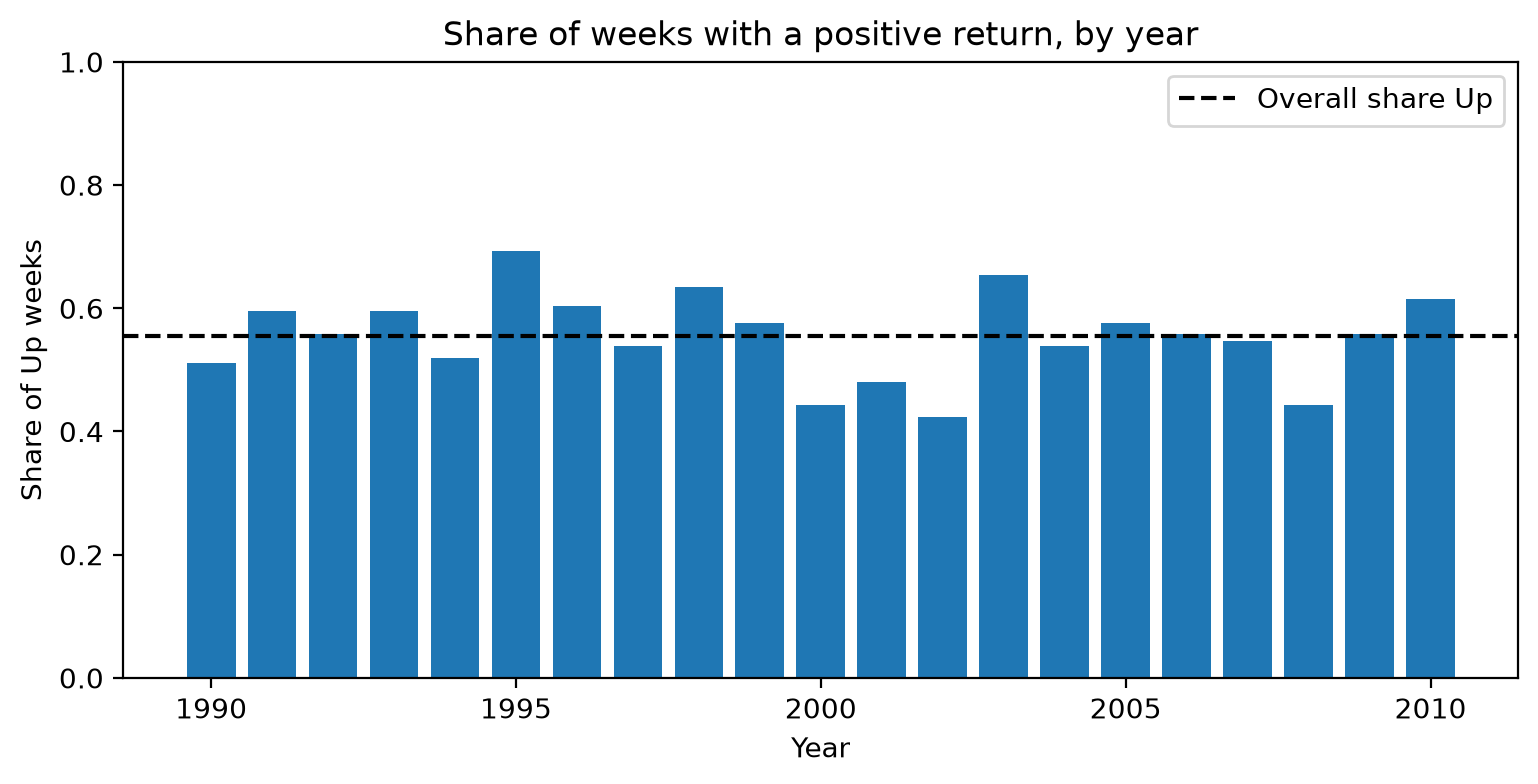
\includegraphics[width=0.8\linewidth]{a2_weekly_up_share.png}
  \caption{Share of Up weeks by year; the dashed line is the overall share.}
\end{figure}

\textbf{Interpretation.} The data contain 1,089 weekly S\&P 500 returns from 1990 to 2010.

\textbf{Distribution of returns.} The mean weekly return is 0.15 \% with a standard deviation of 2.36 \%, so the average week is close to zero relative to its spread. The distribution is not normal: it is more peaked around zero and has much heavier tails than a normal distribution with the same mean and variance (excess kurtosis 5.7, skewness $-$0.48). There are 13 weeks with a return beyond $\pm$3 standard deviations, compared with about 3 expected under normality, and both the largest loss ($-$18.2 \%) and the largest gain (+12.0 \%) occur in 2008. The negative skew means large drops are more extreme than large gains.

\textbf{Volatility.} Volatility is clearly not constant. The 1-year rolling volatility (annualised) ranges from 6.5 \% in early 1994 to 39.1 \% in late 2009, compared with 17.0 \% over the full sample. Calm and turbulent periods cluster: volatility rises through the late 1990s, stays high during the 2000--2002 dot-com crash, falls back to around 10 \% in 2004--2007 and spikes during the 2008 financial crisis. Large moves tend to be followed by large moves, even though their sign is unpredictable.

\textbf{Volume.} The only strong pattern in the data is the trend in Volume, which has a correlation of 0.84 with Year and rises from about 0.15 to 4.6 billion shares per day. On a log scale the increase is roughly linear, so volume has grown approximately exponentially.

\textbf{Predictability of returns.} The lag variables are almost uncorrelated with Today (all correlations between $-$0.075 and 0.059), and Volume is essentially uncorrelated with Today ($-$0.033). The boxplots show that the distributions of the lagged returns overlap almost completely for ``Up'' and ``Down'' weeks. The largest difference is in Lag2, with a mean of 0.30 \% in ``Up'' weeks versus $-$0.04 \% in ``Down'' weeks, which is small compared with the standard deviation of 2.36 \%. Overall, 55.6 \% of weeks are ``Up'', and the share varies between 42 \% and 69 \% across years.

\textbf{Conclusion.} Apart from the upward trend in Volume and the time-varying volatility, there is little evidence of a pattern that would help predict the direction of the market. Past returns carry at most weak information about this week's return, so we should not expect a classifier to do much better than the 55.6 \% accuracy obtained by always predicting ``Up''.

\subsubsection*{(b) Logistic regression on the full data set.}

\begin{table}[H]
  \centering
  \begin{tabular}{lrrrr}
    \toprule
    & Coefficient & Std.\ error & $z$ & $p$-value \\
    \midrule
    Intercept & 0.2669 & 0.086 & 3.106 & 0.002 \\
    \texttt{Lag1} & $-0.0413$ & 0.026 & $-1.563$ & 0.118 \\
    \texttt{Lag2} & 0.0584 & 0.027 & 2.175 & 0.030 \\
    \texttt{Lag3} & $-0.0161$ & 0.027 & $-0.602$ & 0.547 \\
    \texttt{Lag4} & $-0.0278$ & 0.026 & $-1.050$ & 0.294 \\
    \texttt{Lag5} & $-0.0145$ & 0.026 & $-0.549$ & 0.583 \\
    \texttt{Volume} & $-0.0227$ & 0.037 & $-0.616$ & 0.538 \\
    \bottomrule
  \end{tabular}
  \caption{Logistic regression of \texttt{Direction} (Up $=1$) on the five lags and \texttt{Volume}.}
\end{table}

Looking at the p-values for the coefficient estimates, we see that only Lag2 is significant at the 5\% significance level.

\subsubsection*{(c) Confusion matrix and overall fraction of correct predictions.}

\begin{table}[H]
  \centering
  \begin{tabular}{lrr}
    \toprule
    & Truth: Down & Truth: Up \\
    \midrule
    Predicted: Down & 54 & 48 \\
    Predicted: Up & 430 & 557 \\
    \bottomrule
  \end{tabular}
  \caption{Logistic regression from (b), threshold 0.5, full data set. Accuracy 56.11\,\%.}
\end{table}

The confusion matrix is for the logistic regression from (b), with all six predictors and a threshold of 0.5, evaluated on the full data set. It shows the two types of mistakes a classifier can make: false positives and false negatives. If we define ``Up'' as the positive class, a false positive is a week where the model predicts ``Up'' but the actual class is ``Down'', and a false negative is a week where the model predicts ``Down'' but the actual class is ``Up''.

The model is correct in \((557 + 54)/1089 \approx 56.1\%\) of the weeks. This is barely better than the trivial rule of always predicting ``Up'', which is correct in \(605/1089 \approx 55.6\%\) of the weeks. The two types of mistakes are also very unevenly distributed:

\[\text{TPR} = \frac{TP}{P} = \frac{557}{605} \approx 0.921, \qquad \text{TNR} = \frac{TN}{N} = \frac{54}{484} \approx 0.112\]

The model finds 92.1 \% of the ``Up'' weeks but only 11.2 \% of the ``Down'' weeks. Of the 478 misclassified weeks, 430 are false positives and only 48 are false negatives. In other words, the model labels almost every ``Down'' week as ``Up'', and it predicts ``Up'' in 987 of the 1089 weeks.

The reason is the structure of the data. As seen in (a) and (b), the predictors have very weak predictive power: their correlations with Today are close to zero, and only Lag2 is significant. At the same time, ``Up'' is slightly more common than ``Down'' (55.6 \% versus 44.4 \%). With weak predictors, the fitted probability \(\hat P(\text{Up} \mid X)\) stays close to this base rate for almost every week. Its median is 0.557, and half of the weeks lie between 0.528 and 0.582. With a threshold of 0.5, nearly all predictions therefore become ``Up''. The model mostly reproduces the majority class instead of separating the two classes.

\subsubsection*{(d) Logistic regression with \texttt{Lag2}, trained on 1990--2008 and tested on 2009--2010.}

\begin{table}[H]
  \centering
  \begin{tabular}{lrrrr}
    \toprule
    & Coefficient & Std.\ error & $z$ & $p$-value \\
    \midrule
    Intercept & 0.2033 & 0.064 & 3.162 & 0.002 \\
    \texttt{Lag2} & 0.0581 & 0.029 & 2.024 & 0.043 \\
    \bottomrule
  \end{tabular}
  \caption{Logistic regression on the training period 1990--2008.}
\end{table}

\begin{table}[H]
  \centering
  \begin{tabular}{lrr}
    \toprule
    & Truth: Down & Truth: Up \\
    \midrule
    Predicted: Down & 9 & 5 \\
    Predicted: Up & 34 & 56 \\
    \bottomrule
  \end{tabular}
  \caption{Test period 2009--2010 (104 weeks). Accuracy $65/104 = 62.5\,\%$.}
\end{table}

\subsubsection*{(e)--(h) LDA, QDA, KNN with $K = 1$ and naive Bayes.}
All four methods use \texttt{Lag2} as the only predictor and the same training and test periods as in (d).

\begin{table}[H]
  \centering
  \begin{tabular}{lcccc}
    \toprule
    & (e) LDA & (f) QDA & (g) KNN, $K=1$ & (h) Naive Bayes \\
    \midrule
    Predicted Down, truth Down & 9 & 0 & 21 & 0 \\
    Predicted Down, truth Up & 5 & 0 & 30 & 0 \\
    Predicted Up, truth Down & 34 & 43 & 22 & 43 \\
    Predicted Up, truth Up & 56 & 61 & 31 & 61 \\
    \midrule
    Test accuracy & 62.50\,\% & 58.65\,\% & 50.00\,\% & 58.65\,\% \\
    \bottomrule
  \end{tabular}
  \caption{Confusion matrices on the test period 2009--2010.}
\end{table}

\subsubsection*{(i) Which method gives the best results?}

\begin{table}[H]
  \centering
  \small
  \setlength{\tabcolsep}{4pt}
  \begin{tabular}{lrrrrrr}
    \toprule
    & Accuracy & Recall Up & Recall Down & Prec.\ Up & Prec.\ Down & \# pred.\ Down \\
    \midrule
    (d) Logistic & 0.625 & 0.918 & 0.209 & 0.622 & 0.643 & 14 \\
    (e) LDA & 0.625 & 0.918 & 0.209 & 0.622 & 0.643 & 14 \\
    (f) QDA & 0.587 & 1.000 & 0.000 & 0.587 & -- & 0 \\
    (h) Naive Bayes & 0.587 & 1.000 & 0.000 & 0.587 & -- & 0 \\
    Baseline: always Up & 0.587 & 1.000 & 0.000 & 0.587 & -- & 0 \\
    (g) KNN, $K = 1$ & 0.500 & 0.508 & 0.488 & 0.585 & 0.412 & 51 \\
    \bottomrule
  \end{tabular}
  \caption{Test-set metrics, sorted by accuracy. The decision boundaries are $\texttt{Lag2} = -3.50$ (logistic) and $-3.52$ (LDA). A one-sided binomial test of 65/104 against the baseline accuracy 0.587 gives $p = 0.24$.}
\end{table}

\textbf{Metrics.} ``Up'' is treated as the positive class. Recall ``Up'' is the share of actual ``Up'' weeks that were predicted ``Up'', and recall ``Down'' is the same for ``Down'' weeks. Precision is the share of predictions of a class that were correct. Precision ``Down'' is undefined (NaN) for models that never predict ``Down''.

\textbf{Two features of the data explain all the confusion matrices.} First, the signal in Lag2 is very weak. In part (a), Lag2 had a correlation of only 0.06 with Today, and its mean differs by about 0.3 percentage points between ``Up'' and ``Down'' weeks, against a standard deviation of about 2.3. The two class-conditional distributions of Lag2 therefore overlap almost completely, so every model's estimate of P(``Up'' \textbar{} Lag2) stays close to the prior. Second, the classes are imbalanced: 55.2 \% of training weeks and 58.7 \% of test weeks are ``Up''. When the posterior is close to the prior and the prior favours ``Up'', a model with a 0.5 threshold will predict ``Up'' almost everywhere.

\textbf{Logistic regression and LDA (62.5 \%).} With a single predictor, both methods produce a decision rule that is linear in Lag2, so it reduces to one cut-off. The cut-offs are almost identical: ``Down'' is predicted only when Lag2 \textless{} $-$3.50 (logistic) or $-$3.52 (LDA). As a result, the two methods give exactly the same predictions on the test set. They predict ``Down'' only after a large fall two weeks earlier. That happened in 14 of the 104 test weeks, more often than usual because 2009 followed the financial crisis and was unusually volatile. In 9 of those 14 weeks the market did fall (precision ``Down'' 64 \%). The models therefore catch only 9 of the 43 ``Down'' weeks (recall ``Down'' 21 \%) while catching 56 of the 61 ``Up'' weeks (recall ``Up'' 92 \%). Most errors are ``Down'' weeks predicted as ``Up''.

\textbf{QDA and naive Bayes (58.7 \%).} With one predictor, the naive Bayes independence assumption is irrelevant, so Gaussian naive Bayes is the same model as QDA and the two confusion matrices are identical. The estimated variance of Lag2 is larger for ``Up'' weeks than for ``Down'' weeks, so ``Up'' wins in both tails. In the middle, the class means are so close that ``Down'' never overcomes the larger prior of ``Up''. The estimated P(``Up'') is above 0.5 for every value of Lag2, so both models predict ``Up'' for every week (recall ``Up'' 100 \%, recall ``Down'' 0 \%). Their accuracy equals the share of ``Up'' weeks in the test period: they do no better than the trivial baseline.

\textbf{KNN with K = 1 (50.0 \%).} KNN with K = 1 is the most flexible method and has the highest variance: each prediction copies the label of the single nearest training week. Because the classes overlap almost completely in Lag2, that label is close to a coin flip. KNN is the only method that predicts ``Down'' often (51 times), and its recalls for both classes are about 50 \%. It ignores the class imbalance and fits noise, so it ends up below the baseline.

\textbf{Conclusion.} Logistic regression and LDA give the best results (62.5 \% accuracy, the highest precision for both classes and the only non-trivial recall for ``Down''). However, the improvement over always predicting ``Up'' is only 4 weeks out of 104. A one-sided binomial test against the baseline accuracy of 58.7 \% gives p = 0.24, so the difference could easily be due to chance. This agrees with part (a): past returns carry little information about the direction of the market, and the simple linear methods win mainly because they do not try to fit structure that is not there.

\subsubsection*{(j) Other combinations of predictors and methods.}

\begin{table}[H]
  \centering
  \small
  \begin{tabular}{llrrrr}
    \toprule
    Predictors & Method & Accuracy & Recall Up & Recall Down & Balanced acc. \\
    \midrule
    \multicolumn{6}{l}{\emph{Top 5 by accuracy}} \\
    \texttt{Lag2} & Logistic & 0.625 & 0.918 & 0.209 & 0.564 \\
    \texttt{Lag2} & LDA & 0.625 & 0.918 & 0.209 & 0.564 \\
    \texttt{Lag2} + \texttt{Lag2}$^2$ & Logistic & 0.625 & 0.934 & 0.186 & 0.560 \\
    \texttt{Lag2} + \texttt{Lag2}$^2$ & QDA & 0.625 & 0.951 & 0.163 & 0.557 \\
    \texttt{Lag2} + \texttt{Lag2}$^2$ & LDA & 0.615 & 0.934 & 0.163 & 0.549 \\
    \midrule
    \multicolumn{6}{l}{\emph{Top 5 by balanced accuracy}} \\
    \texttt{Lag2} & KNN, $K = 20$ & 0.596 & 0.639 & 0.535 & 0.587 \\
    \texttt{Lag2} + \texttt{Lag2}$^2$ & KNN, $K = 20$ & 0.596 & 0.639 & 0.535 & 0.587 \\
    \texttt{Lag2} + log \texttt{Volume} & KNN, $K = 1$ & 0.567 & 0.525 & 0.628 & 0.576 \\
    \texttt{Lag2} + \texttt{Lag2}$^2$ & KNN, $K = 50$ & 0.577 & 0.607 & 0.535 & 0.571 \\
    \texttt{Lag1}--\texttt{Lag5} & KNN, $K = 10$ & 0.567 & 0.557 & 0.581 & 0.569 \\
    \bottomrule
  \end{tabular}
  \caption{Best of the 60 combinations (6 predictor sets $\times$ 10 methods) on the test period 2009--2010.}
\end{table}

\textbf{Interpretation.} We tried six sets of predictors with five methods (Logistic regression, LDA, QDA, naive Bayes and KNN), using \(K \in \{1, 5, 10, 20, 50, 100\}\) for KNN. That gives 60 combinations, all trained on 1990--2008 and evaluated on the held-out weeks of 2009--2010.

\textbf{Best result.} The highest test accuracy is 62.5 \%. Four combinations reach it: logistic regression and LDA with Lag2 alone, and logistic regression and QDA with Lag2 and Lag2$^2$. We report \textbf{logistic regression with Lag2} as the best model because it is the simplest of them. Its confusion matrix is

\begin{center}
\begin{tabular}{lrr}
\toprule
& Truth: Down & Truth: Up \\
\midrule
Predicted: Down & 9 & 5 \\
Predicted: Up & 34 & 56 \\
\bottomrule
\end{tabular}
\end{center}

This is the same model as in (d), so none of the transformations, interactions or additional predictors improved on it. The model predicts Down only 14 times. It finds 92 \% of the Up weeks but only 21 \% of the Down weeks, so its high accuracy comes mainly from predicting the majority class.

\textbf{Adding predictors does not help.} For the linear methods, adding Lag1, the interaction Lag1$\cdot$Lag2, log Volume or all five lags lowers the test accuracy from 62.5 \% to between 54.8 \% and 57.7 \%. These variables have almost no relationship with Direction (see (a) and (b)), so they mainly add estimation noise. The flexible methods suffer most. QDA and naive Bayes with the interaction term or with all five lags fall to 46--48 \%, well below the 58.7 \% obtained by always predicting Up. Only 10 of the 60 combinations beat that baseline, and 50 do worse.

\textbf{KNN.} Test accuracy for KNN varies irregularly with \(K\), between 43 \% and 60 \%, with no clear trend. This is what we would expect when the classes overlap almost completely: small changes in \(K\) or in the predictors change which neighbours are used, and the result is mostly noise. Larger \(K\) makes KNN predict Up more often (with \(K = 100\) it predicts Down only 22--38 times), so it moves towards the majority-class rule. The best KNN model is \(K = 20\) with Lag2, at 59.6 \%.

\textbf{Choice of metric.} Accuracy rewards models that lean on the majority class. If we instead rank by balanced accuracy, the average of recall Up and recall Down, the best model is KNN with \(K = 20\) and Lag2 (balanced accuracy 0.587, versus 0.564 for logistic regression). It finds 23 of the 43 Down weeks (53 \%) instead of 9, at the cost of more misclassified Up weeks. If the goal is to avoid losses, for example by not investing before a fall, this model may be more useful even though its overall accuracy is lower.

\textbf{Caveat.} The best model was chosen among 60 combinations based on only 104 test weeks, so its accuracy is likely somewhat optimistic. The winning margin over always predicting Up is 4 weeks, which is not statistically significant (one-sided binomial test, \(p = 0.24\)). The overall conclusion is the same as in (a) and (i): past returns and volume contain very little information about next week's direction, and the simplest model with the single most informative predictor performs as well as anything more complex.

\begin{table}[H]
  \centering
  \begin{tabular}{lrr}
    \toprule
    & Truth: Down & Truth: Up \\
    \midrule
    Predicted: Down & 23 & 22 \\
    Predicted: Up & 20 & 39 \\
    \bottomrule
  \end{tabular}
  \caption{KNN with $K = 20$ and \texttt{Lag2}, the best model by balanced accuracy.}
\end{table}

% ----------------------------------------------------------------------------
\subsection*{Exercise 14 -- \texttt{Auto}}

\subsubsection*{(a)--(b) The variable \texttt{mpg01} and its association with the other features}
\texttt{mpg01} is 1 if \texttt{mpg} is above its median (22.75) and 0 otherwise, so exactly half of the 392 cars have \texttt{mpg01} $= 1$.

\begin{figure}[H]
  \centering
  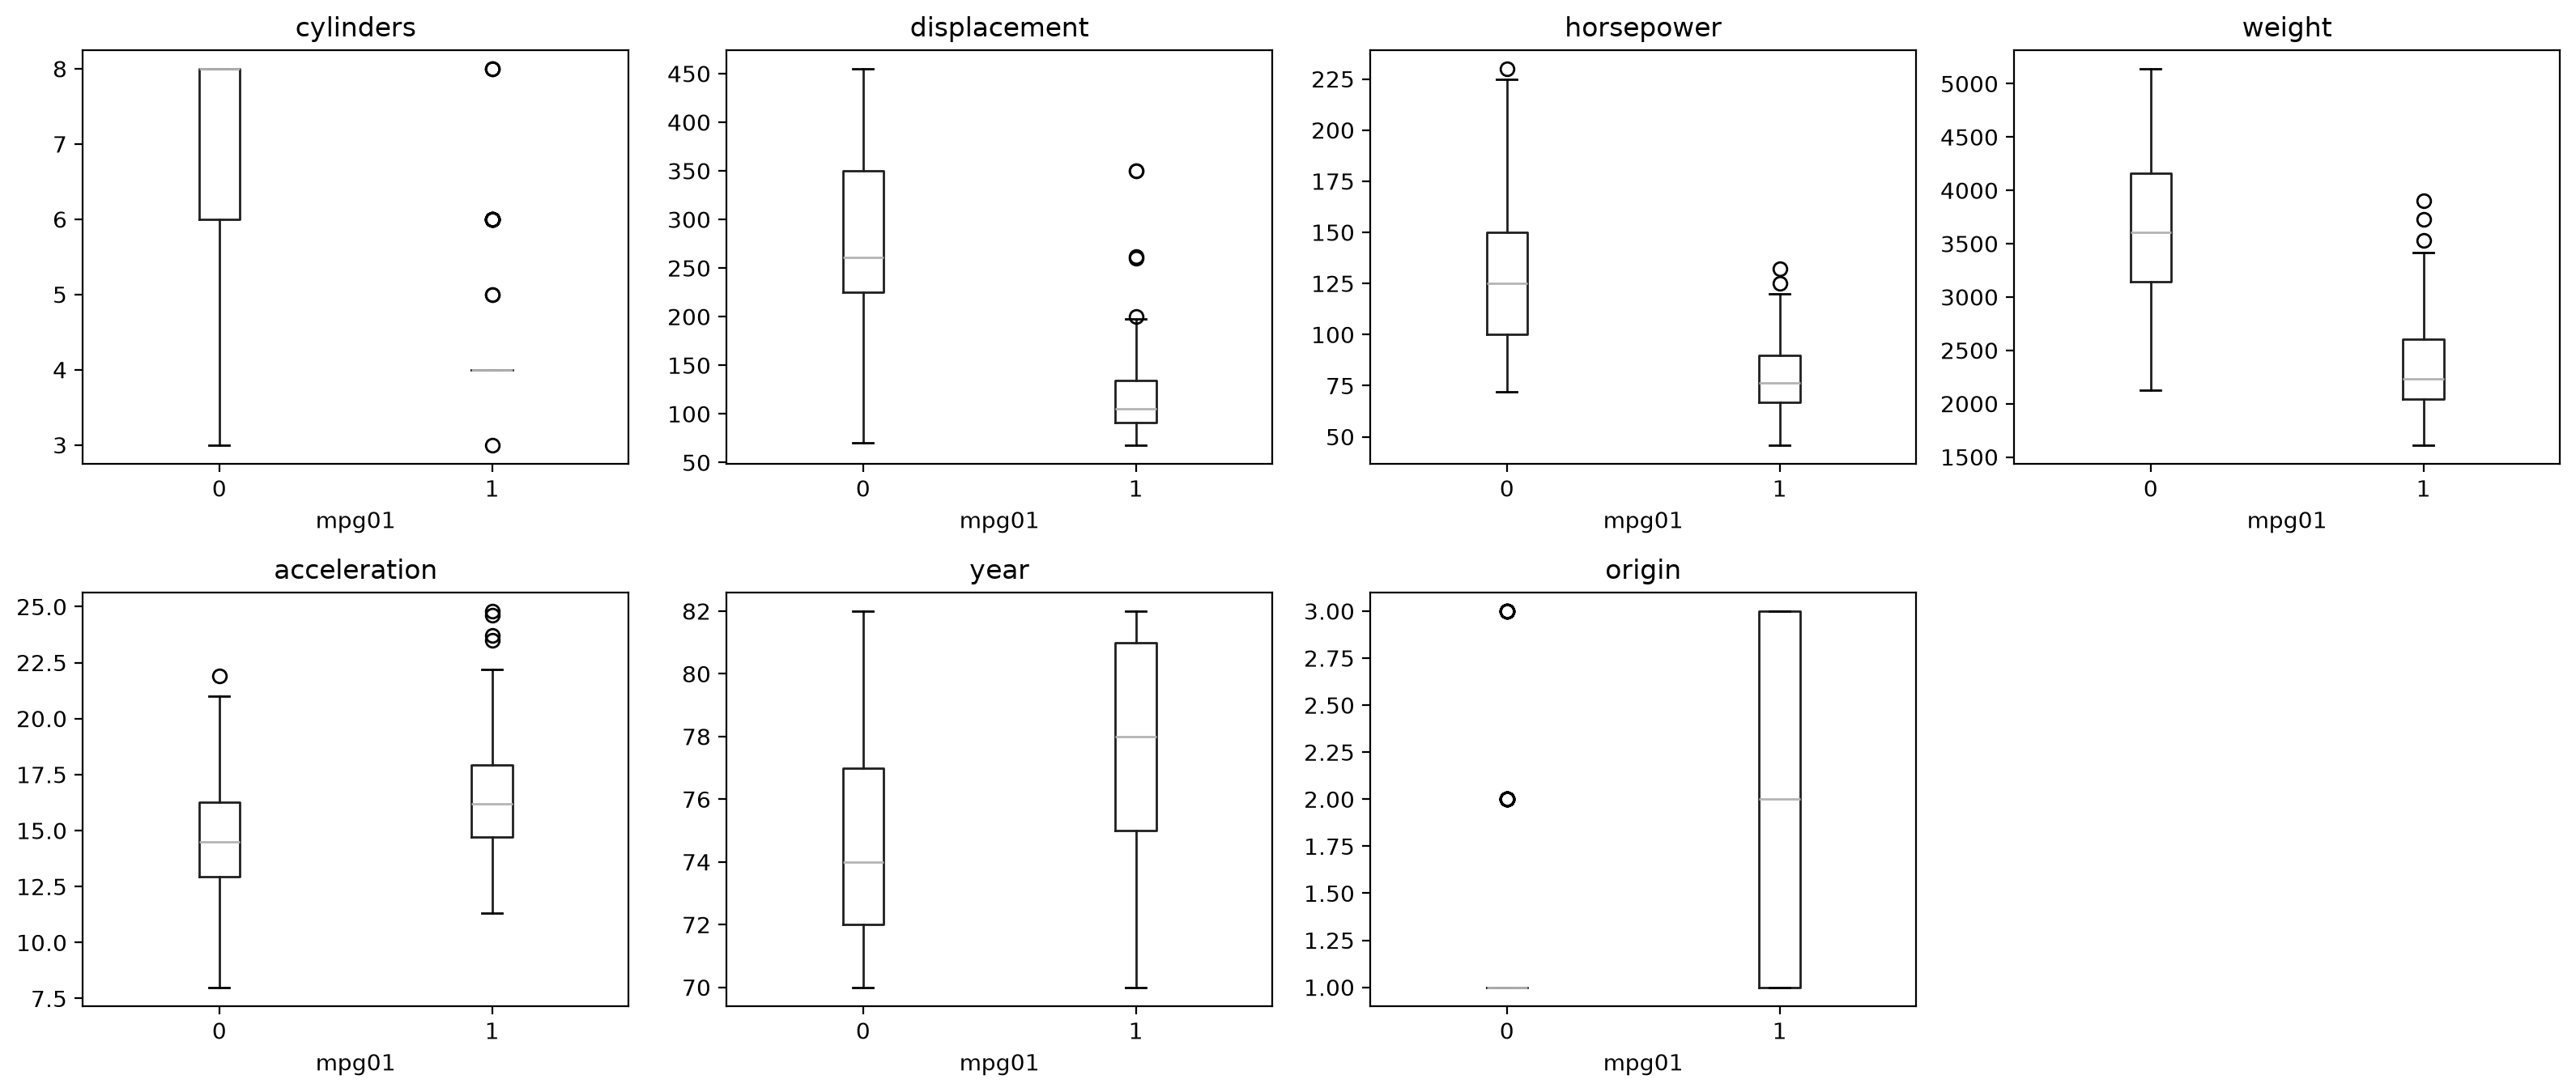
\includegraphics[width=\linewidth]{a2_auto_boxplots.png}
  \caption{Each feature by \texttt{mpg01}.}
\end{figure}

\begin{figure}[H]
  \centering
  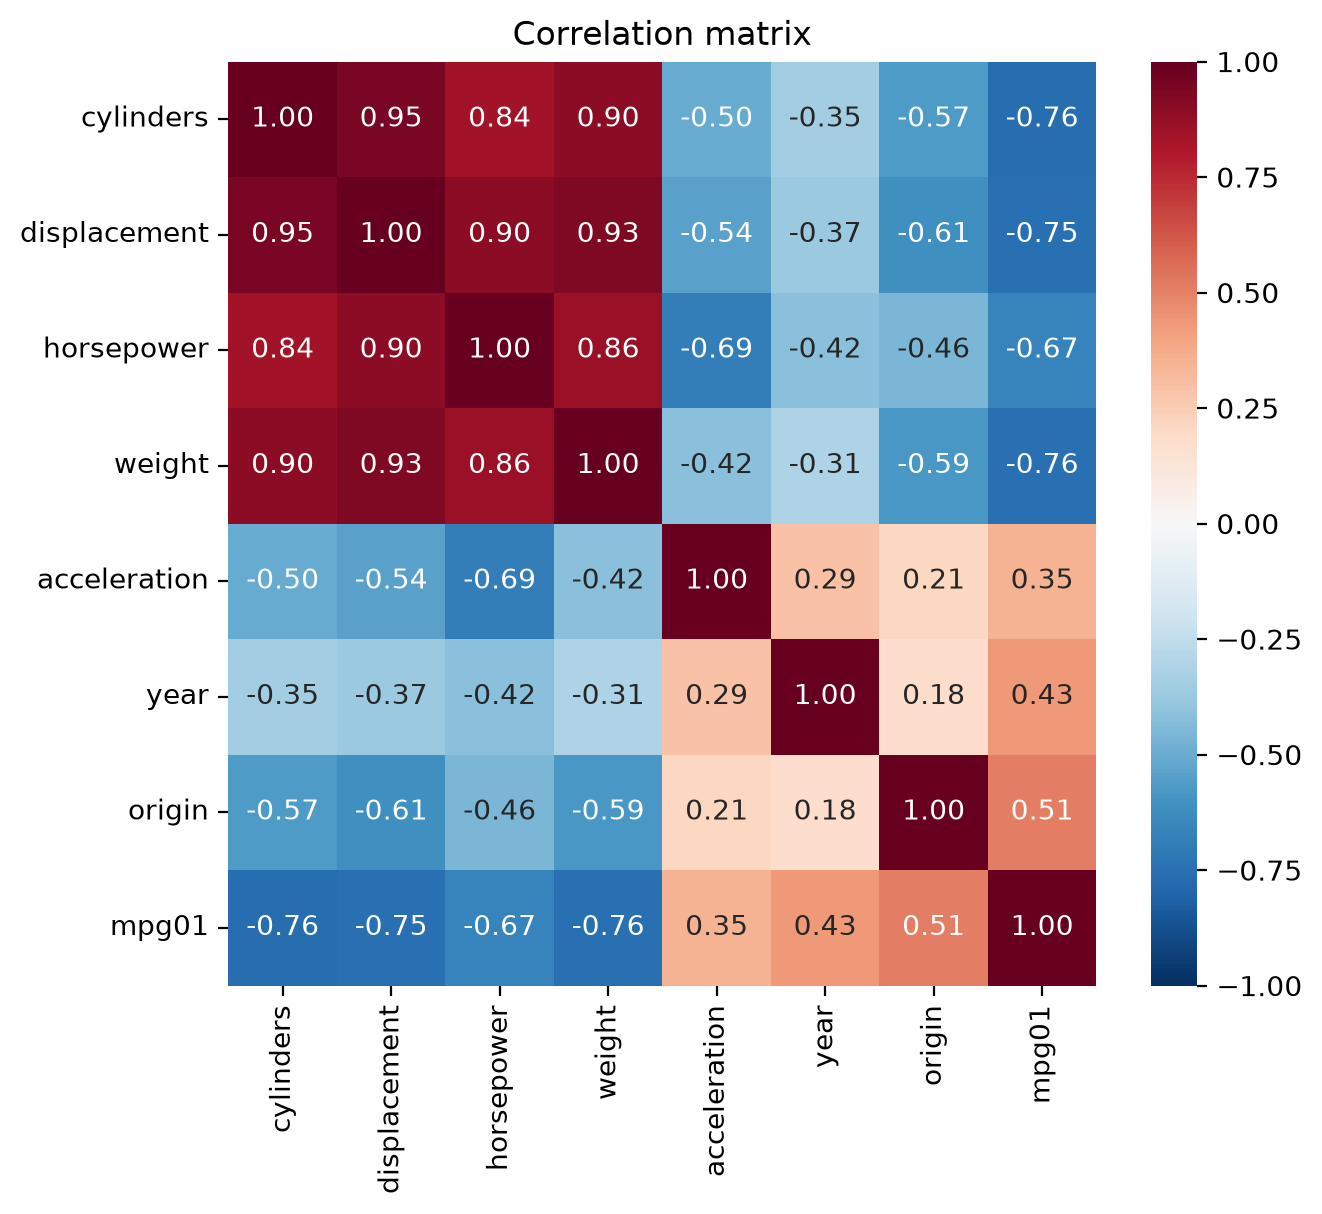
\includegraphics[width=0.6\linewidth]{a2_auto_corr.png}
  \caption{Correlation matrix of \texttt{Auto} without \texttt{mpg}.}
\end{figure}

\begin{table}[H]
  \centering
  \begin{tabular}{lr}
    \toprule
    Feature & Correlation with \texttt{mpg01} \\
    \midrule
    \texttt{cylinders} & $-0.759$ \\
    \texttt{weight} & $-0.758$ \\
    \texttt{displacement} & $-0.753$ \\
    \texttt{horsepower} & $-0.667$ \\
    \texttt{acceleration} & 0.347 \\
    \texttt{year} & 0.430 \\
    \texttt{origin} & 0.514 \\
    \bottomrule
  \end{tabular}
\end{table}

\subsubsection*{(c)--(h) Training and test sets; LDA, QDA, logistic regression, naive Bayes and KNN}
The data are split into a training set (70\,\%) and a test set (30\,\%, 118 cars), stratified on \texttt{mpg01} (\texttt{random\_state = 0}). Eleven sets of predictors are combined with LDA, QDA, logistic regression, naive Bayes and KNN with $K \in \{1, 5, 10, 20, 50, 100\}$, which gives 110 models. One misclassified car corresponds to a test error of $1/118 \approx 0.0085$.

\begin{table}[H]
  \centering
  \begin{tabular}{llcr}
    \toprule
    Predictors & Method & \# predictors & Test error \\
    \midrule
    \texttt{displacement}, \texttt{year} & KNN, $K = 5$ & 2 & 0.0763 \\
    \texttt{displacement}, \texttt{year} & Logistic & 2 & 0.0847 \\
    \texttt{cylinders}, \texttt{displacement}, \texttt{horsepower}, \texttt{weight} & KNN, $K = 5$ & 4 & 0.0847 \\
    the four above $+$ \texttt{year} & KNN, $K = 1$ & 5 & 0.0847 \\
    \texttt{displacement}, \texttt{year} & KNN, $K = 1$ & 2 & 0.0932 \\
    \texttt{weight}, \texttt{horsepower}, \texttt{year} & KNN, $K = 5$ & 3 & 0.1017 \\
    \texttt{displacement}, \texttt{year} & Naive Bayes & 2 & 0.1017 \\
    \texttt{weight}, \texttt{year} & KNN, $K = 20$ & 2 & 0.1017 \\
    \texttt{weight}, \texttt{year} & KNN, $K = 10$ & 2 & 0.1017 \\
    \texttt{cylinders}, \texttt{displacement}, \texttt{horsepower}, \texttt{weight} & KNN, $K = 1$ & 4 & 0.1017 \\
    \bottomrule
  \end{tabular}
  \caption{The ten models with the lowest test error out of 110.}
\end{table}

\begin{table}[H]
  \centering
  \begin{tabular}{lrr}
    \toprule
    Method & Test error & Misclassified (of 118) \\
    \midrule
    (d) LDA & 0.1271 & 15 \\
    (e) QDA & 0.1102 & 13 \\
    (f) Logistic regression & 0.0847 & 10 \\
    (g) Naive Bayes & 0.1017 & 12 \\
    (h) KNN, $K = 1$ & 0.0932 & 11 \\
    (h) KNN, $K = 5$ & 0.0763 & 9 \\
    (h) KNN, $K = 10$ & 0.1102 & 13 \\
    (h) KNN, $K = 20$ & 0.1271 & 15 \\
    (h) KNN, $K = 50$ & 0.1186 & 14 \\
    (h) KNN, $K = 100$ & 0.1186 & 14 \\
    \bottomrule
  \end{tabular}
  \caption{Test error of each method with the predictors \texttt{displacement} and \texttt{year}.}
\end{table}

For this data, we get the best performance with $K = 5$ and using displacement and years as predictors.

% ============================================================================
\section*{Chapter 5}

\subsection*{Exercise 1}
\handwritten{ch5_ex1.jpg,ch5_ex1.png,1.png}

% ----------------------------------------------------------------------------
\subsection*{Exercise 2}

\subsubsection*{(a)--(f)}
\handwritten{ch5_ex2.jpg,ch5_ex2.png,2.png}

\subsubsection*{(g)}

\begin{figure}[H]
  \centering
  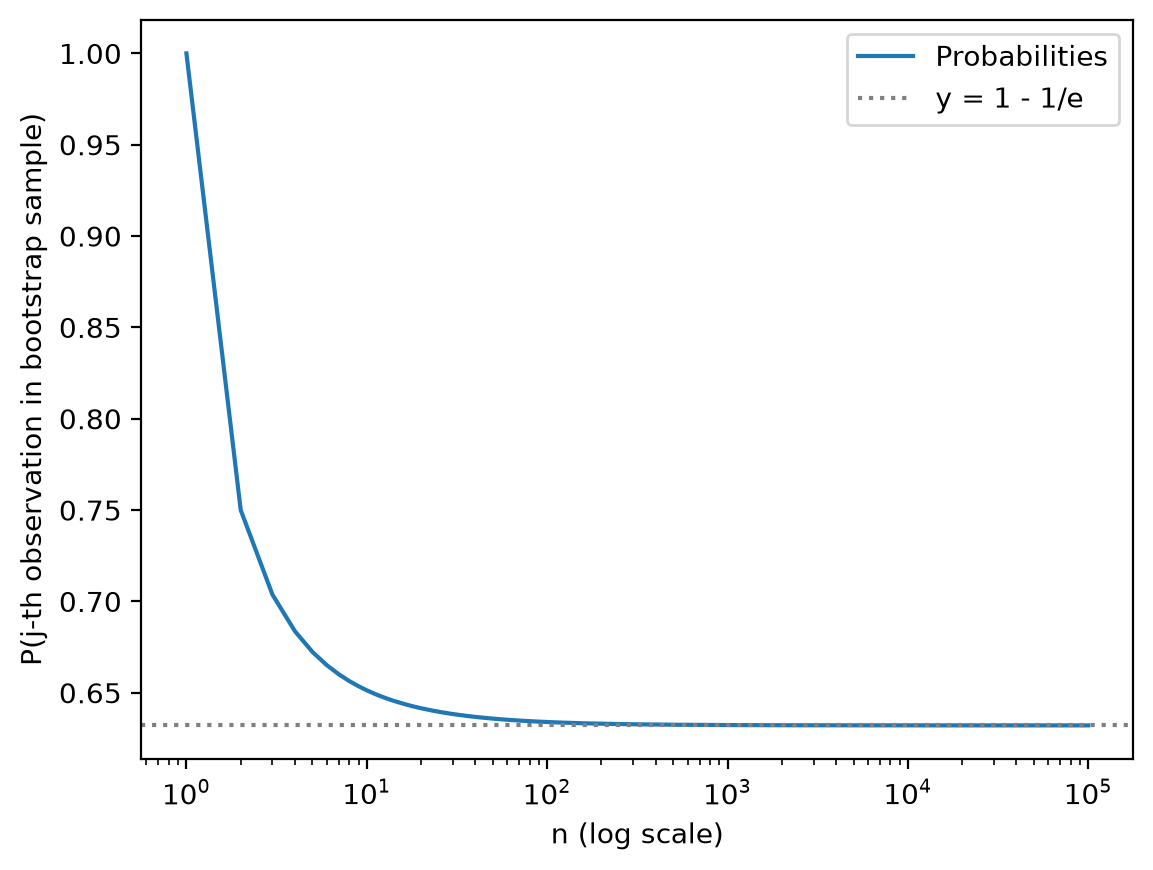
\includegraphics[width=0.7\linewidth]{a2_bootstrap_prob.png}
  \caption{Probability that the $j$th observation is in a bootstrap sample of size $n$, $1 - (1 - 1/n)^n$, for $n = 1, \dots, 100\,000$ (logarithmic $x$-axis). The dotted line is the limit $1 - 1/e \approx 0.632$.}
\end{figure}

We see that the probability that a specific observation in the original sample is in the bootstrap sample converges to $1 - \frac{1}{e}$. When the original sample is small the probability of drawing a specific observation during the bootstrapping process is higher. If we denote the original sample as $\{X_i\}_{i=1,\dots,n}$ and the bootstrap sample as $\{Y_i\}_{i=1,\dots,n}$, then
\[
  P(Y_i = X_j) = \frac{1}{n}
\]
and the probability that a bootstrap observation is not equal to a specific observation is
\[
  P(Y_i \neq X_j) = 1 - \frac{1}{n}.
\]
However, when you increase the size of the sample, and therefore the size of the bootstrap sample, you also increase the number of opportunities to draw that observation. As the bootstrap sampling is done with replacement, all the observations are independent identically distributed random variables. Thus, the joint probability that a specific observation is not in the bootstrap sample is
\[
  P(Y_1 \neq X_j \cap \dots \cap Y_n \neq X_j) = \left(1 - \frac{1}{n}\right)^n.
\]
The probability that at least one of the bootstrap observations is equal to the specific observation is the complement of the previous probability. Taking the limit as the sample size goes to infinity gives
\[
  \lim_{n \to \infty} P(\exists\, i : Y_i = X_j) = 1 - \frac{1}{e}.
\]

\subsubsection*{(h)}

In 10\,000 bootstrap samples of size $n = 100$, drawn with replacement, observation $j = 4$ was included in a share of $0.6362$ of the samples. The exact probability from (e) is $1 - (1 - 1/100)^{100} \approx 0.6340$.

The simulated share agrees closely with the exact probability; the small difference is Monte Carlo variation from using 10\,000 repetitions. We see that the convergence towards the limit is fast.

% ----------------------------------------------------------------------------
\subsection*{Exercise 5 -- \texttt{Default}}

\subsubsection*{(a) Logistic regression of \texttt{default} on \texttt{income} and \texttt{balance}.}

\begin{table}[H]
  \centering
  \begin{tabular}{lr}
    \toprule
    & Coefficient \\
    \midrule
    Intercept & $-11.54$ \\
    \texttt{income} & $2.081 \times 10^{-5}$ \\
    \texttt{balance} & $5.647 \times 10^{-3}$ \\
    \bottomrule
  \end{tabular}
  \caption{Fitted on all 10\,000 observations.}
\end{table}

\subsubsection*{(b) Validation set approach.}
With a 50/50 split (\texttt{random\_state = 0}), the model is fitted on the training half and an observation in the validation half is classified as a default if $\hat P(\texttt{default} = \text{Yes} \mid X) > 0.5$. The validation set error is $0.0290$ (2.90\,\%).

\subsubsection*{(c) Three different splits.}

\begin{table}[H]
  \centering
  \begin{tabular}{crr}
    \toprule
    \texttt{random\_state} & Validation error & Share of defaults in validation set \\
    \midrule
    0 & 0.0290 & 0.0372 \\
    1 & 0.0250 & 0.0318 \\
    2 & 0.0248 & 0.0308 \\
    \bottomrule
  \end{tabular}
\end{table}

\textbf{Interpretation (c).} The validation set error depends on how the data is split. With three random splits it is 2.90 \%, 2.50 \% and 2.48 \% (mean $\approx$ 2.63 \%). The gap between the highest and lowest estimate is 21 misclassified observations out of 5000. The split with the highest error also has the most defaults in its validation set (3.72 \% versus about 3.1 \%), which makes sense because almost all errors are defaults that the model misses. The estimate of the test error is therefore variable, which is a known weakness of the validation set approach.

The numbers also need context. Only about 3.3 \% of all customers default, so a classifier that always predicts ``No'' would already have an error of roughly 3.1--3.7 \% on these validation sets. The logistic model is only slightly better. Finally, each model is fitted on just half of the observations, so the validation error tends to overestimate the test error of a model fitted on the full data set. Cross-validation addresses both issues.

\subsubsection*{(d) Adding a dummy variable for \texttt{student}.}

\begin{table}[H]
  \centering
  \begin{tabular}{crrr}
    \toprule
    \texttt{random\_state} & Without \texttt{student} & With \texttt{student} & Share of defaults \\
    \midrule
    0 & 0.0290 & 0.0292 & 0.0372 \\
    1 & 0.0250 & 0.0262 & 0.0318 \\
    2 & 0.0248 & 0.0254 & 0.0308 \\
    \midrule
    Mean & 0.0263 & 0.0269 & 0.0333 \\
    \bottomrule
  \end{tabular}
  \caption{Validation set error on the same three splits as in (c).}
\end{table}

\textbf{Interpretation (d).} Adding the dummy variable for \texttt{student} does not reduce the validation set error. On the same three splits as in (c) the error is 2.92 \%, 2.62 \% and 2.54 \% (mean $\approx$ 2.69 \%), compared with 2.90 \%, 2.50 \% and 2.48 \% (mean $\approx$ 2.63 \%) without it. That is 1--6 more misclassified observations out of 5000, which is smaller than the variation between splits in (c). The difference is therefore best seen as noise and not as a real deterioration.

% ----------------------------------------------------------------------------
\subsection*{Exercise 6 -- Standard errors by \texttt{sm.GLM()} and the bootstrap}

\subsubsection*{(a) Standard errors from \texttt{sm.GLM()}.}

\begin{table}[H]
  \centering
  \begin{tabular}{lrrrr}
    \toprule
    & Coefficient & Std.\ error & $z$ & $p$-value \\
    \midrule
    Intercept & $-11.54$ & 0.4348 & $-26.544$ & $< 0.001$ \\
    \texttt{income} & $2.081 \times 10^{-5}$ & $4.985 \times 10^{-6}$ & 4.174 & $< 0.001$ \\
    \texttt{balance} & $5.647 \times 10^{-3}$ & $2.274 \times 10^{-4}$ & 24.835 & $< 0.001$ \\
    \bottomrule
  \end{tabular}
  \caption{Logistic regression of \texttt{default} on \texttt{income} and \texttt{balance}, fitted with \texttt{sm.GLM()}.}
\end{table}

\subsubsection*{(b) The function \texttt{boot\_fn()}.}

\begin{lstlisting}[language=Python]
def boot_fn(D, idx):
    D_ = D.loc[idx]                                   # the bootstrap sample of D is denoted D_
    X_ = MS(["income", "balance"]).fit_transform(D_)
    y_ = D_["default"] == "Yes"
    fit = sm.GLM(y_, X_, family=sm.families.Binomial()).fit()
    return fit.params[["income", "balance"]]
\end{lstlisting}

\subsubsection*{(c) Bootstrap standard errors.}
Using the function \texttt{boot\_SE()} from the lab with $B = 1000$ bootstrap samples of size $n = 10\,000$, drawn with replacement (\texttt{seed = 0}):

\begin{table}[H]
  \centering
  \begin{tabular}{lr}
    \toprule
    & Bootstrap SE \\
    \midrule
    \texttt{income} & $4.767 \times 10^{-6}$ \\
    \texttt{balance} & $2.304 \times 10^{-4}$ \\
    \bottomrule
  \end{tabular}
\end{table}

\subsubsection*{(d) Comparison.}

\begin{table}[H]
  \centering
  \begin{tabular}{lrrr}
    \toprule
    & \texttt{sm.GLM()} SE & Bootstrap SE & Ratio \\
    \midrule
    \texttt{income} & $4.985 \times 10^{-6}$ & $4.767 \times 10^{-6}$ & 0.956 \\
    \texttt{balance} & $2.274 \times 10^{-4}$ & $2.304 \times 10^{-4}$ & 1.013 \\
    \bottomrule
  \end{tabular}
\end{table}

\textbf{Interpretation (d).} The two methods give very similar standard errors. For \texttt{balance} the bootstrap estimate is about 1 \% larger than the \texttt{sm.GLM()} estimate (2.30e-04 vs 2.27e-04), and for \texttt{income} it is about 4 \% smaller (4.77e-06 vs 4.99e-06). Both differences are small compared with the coefficients themselves, so the conclusions about significance do not change.

The \texttt{sm.GLM()} standard errors come from maximum likelihood theory. They assume that the logistic model is correctly specified and rely on a large-sample approximation. The bootstrap makes no such assumptions; it estimates the variability directly by refitting the model on 1000 resamples of the data. That the two agree so closely suggests that the logistic model with \texttt{income} and \texttt{balance} is a reasonable description of the data, and that the formula-based standard errors can be trusted here. The small remaining differences are partly due to Monte Carlo error from using a finite number of bootstrap samples (B = 1000); a different seed would change the bootstrap estimates slightly.

\end{document}
